\documentclass{beamer}
\mode<presentation>
\usetheme{CambridgeUS}
\usepackage[russian]{babel}
\usepackage[utf8]{inputenc}
\usepackage[T2A]{fontenc}
\usepackage{sansmathaccent}

\usepackage{verbatim}
\usepackage{alltt}

\pdfmapfile{+sansmathaccent.map}
\title[Software Design]{Наследование и иерархии классов}
\author{Наумов Д.А., доц. каф. КТ}
\date[30.09.2019] {Основы программной инженерии, 2019}

\begin{document}

%ТИТУЛЬНЫЙ СЛАЙД
\begin{frame}
  \titlepage
\end{frame}
  
%СОДЕРЖАНИЕ ЛЕКЦИИ
\begin{frame}
  \frametitle{Содержание лекции}
  \tableofcontents  
\end{frame}

\section{Класс как элемент абстракции}

\subsection{Неявный параметр self}
\begin{frame}{Неявный параметр self}
Для доступа к объекту класса, для которого вызван метод, в языке Pascal
существует идентификатор \textbf{self}, обозначающее неявно передаваемый в метод объект.
\begin{figure}[h]
\centering
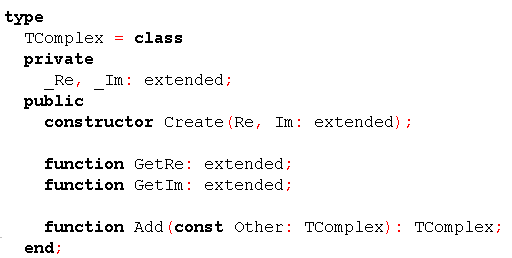
\includegraphics[scale=0.45]{images/lec06-pic01.png}
\end{figure}
При использовании идентификатора self метод выглядит следующим образом:
\begin{figure}[h]
\centering
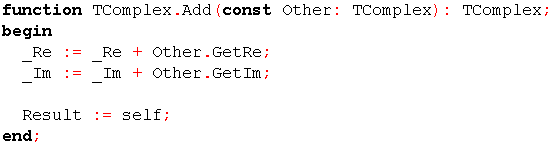
\includegraphics[scale=0.45]{images/lec06-pic02.png}
\end{figure}
\end{frame}

\begin{frame}{Неявный параметр self}
Пример использования метода Add:
\begin{figure}[h]
\centering
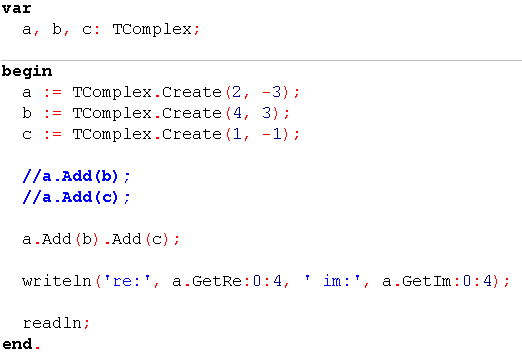
\includegraphics[scale=0.5]{images/lec06-pic03.png}
\end{figure}
\end{frame}

\subsection{Перегрузка методов}
\begin{frame}{Перегрузка методов}
Перегруженные методы используются, когда функции выполняют схожие по смыслу действий задачи с данными различных типов.
\begin{figure}[h]
\centering
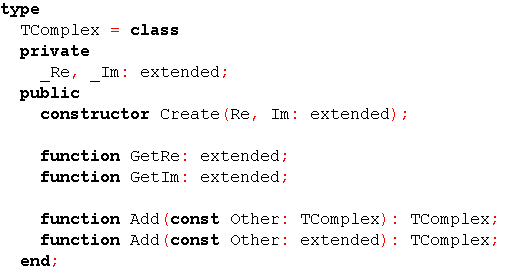
\includegraphics[scale=0.4]{images/lec06-pic04.png}
\end{figure}
Реализация метода:
\begin{figure}[h]
\centering
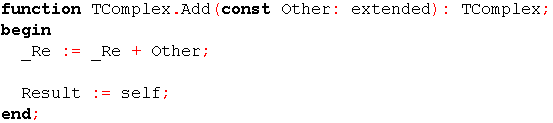
\includegraphics[scale=0.4]{images/lec06-pic05.png}
\end{figure}
Обращение к методу:
\begin{figure}[h]
\centering
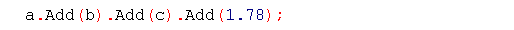
\includegraphics[scale=0.4]{images/lec06-pic06.png}
\end{figure}
\end{frame}

\subsection{Перегрузка арифметических операций}
\begin{frame}{Перегрузка арифметических операций}
Перегрузка арифметических операций полезна тогда, когда хочется обеспечить привычную форму записи выражений при манипуляции с данными
пользовательских типов. 
\begin{figure}[h]
\centering
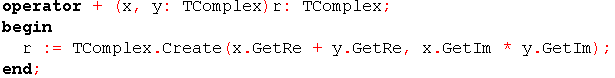
\includegraphics[scale=0.5]{images/lec06-pic07.png}
\end{figure}
Запись выражений, оперирующих данными пользовательских типов в форме, привычной для выражений, оперирующих со встроенными типами, может в ряде случае обеспечивать более наглядный и естественный код.
\begin{figure}[h]
\centering
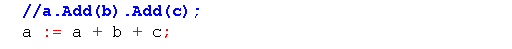
\includegraphics[scale=0.6]{images/lec06-pic08.png}
\end{figure}
\end{frame}

\begin{frame}{Поверхностное копирование объектов}
В результате присваивания значение указателя value объекта mstr2
будет указывать на ту же память, что и указатель value объекта mstri:
\begin{figure}[h]
\centering
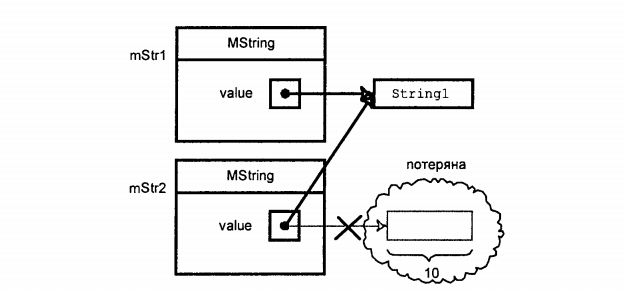
\includegraphics[scale=0.4]{images/lec06-pic09.png}
\end{figure}
Пример:
\begin{figure}[h]
\centering
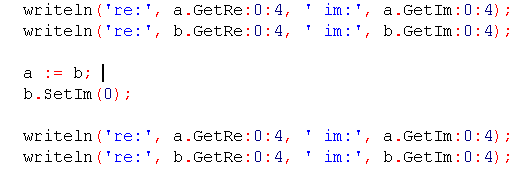
\includegraphics[scale=0.5]{images/lec06-pic10.png}
\end{figure}
\end{frame}
  
\section{Наследование и иерархии классов}

\begin{frame}{Использование агрегации}
Выстраивание иерархии классов на основе отношения агрегации:
\begin{figure}[h]
\centering
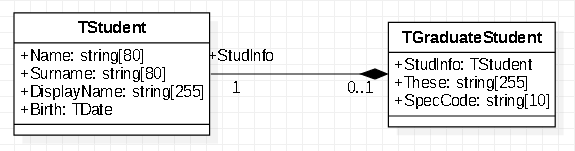
\includegraphics[scale=0.4]{images/lec06-pic11.png}
\end{figure}
Код:
\begin{figure}[h]
\centering
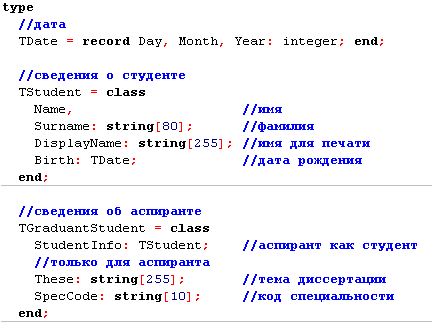
\includegraphics[scale=0.4]{images/lec06-pic12.png}
\end{figure}
Недостатки: тип TGraduateStudent является независимым, его нельзя трактовать как разновидность типа TStudent.
\end{frame}

\subsection{Наследование как основная форма отношения обобщения}
\begin{frame}{Использование наследования}
Объект типа TGraduateStudent является разновидностью объекта TStudent:
\begin{figure}[h]
\centering
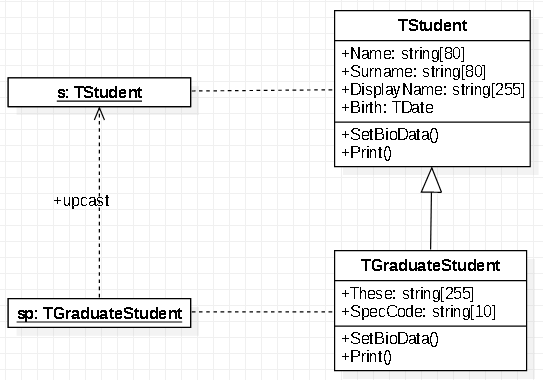
\includegraphics[scale=0.5]{images/lec06-pic13.png}
\end{figure}
\end{frame}

\begin{frame}{Использование наследования}
\begin{figure}[h]
\centering
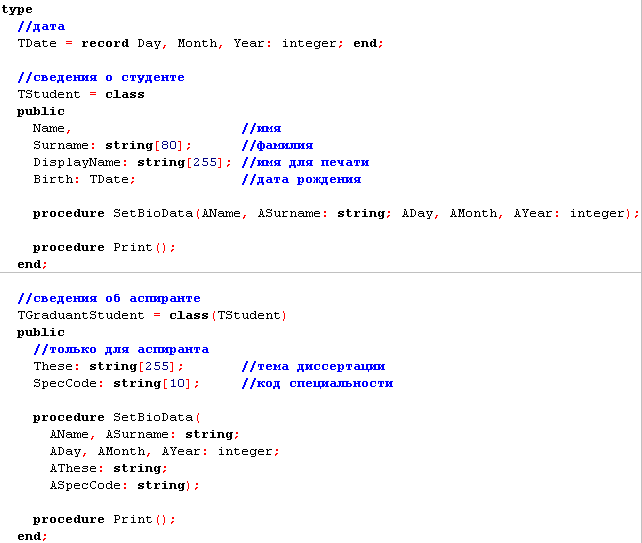
\includegraphics[scale=0.5]{images/lec06-pic14.png}
\end{figure}
\end{frame}

\begin{frame}{Использование наследования}
\begin{figure}[h]
\centering
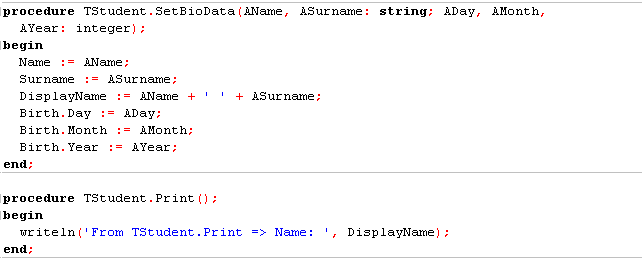
\includegraphics[scale=0.6]{images/lec06-pic15.png}
\end{figure}
\end{frame}

\begin{frame}{Использование наследования}
\begin{figure}[h]
\centering
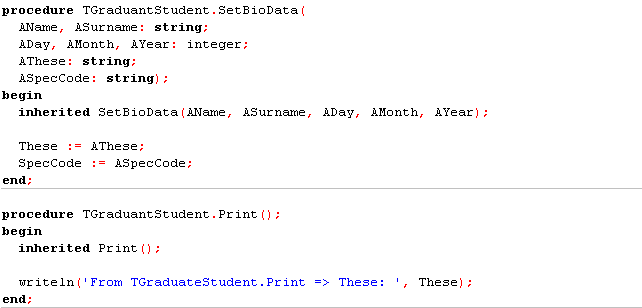
\includegraphics[scale=0.6]{images/lec06-pic16.png}
\end{figure}
\end{frame}

\begin{frame}{Использование наследования}
\begin{figure}[h]
\centering
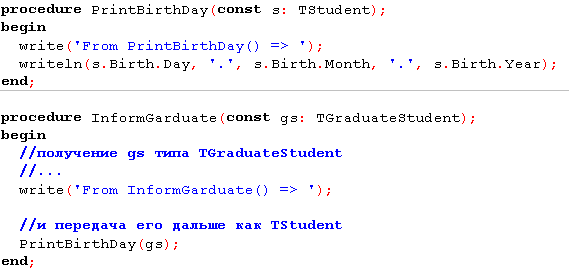
\includegraphics[scale=0.6]{images/lec06-pic17.png}
\end{figure}
\end{frame}

\begin{frame}{Использование наследования}
\begin{figure}[h]
\centering
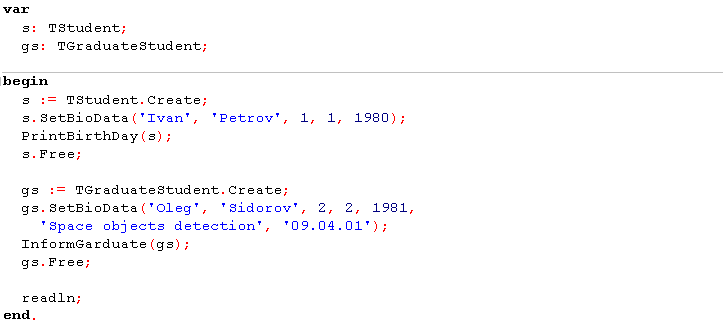
\includegraphics[scale=0.6]{images/lec06-pic18.png}
\end{figure}
\begin{figure}[h]
\centering
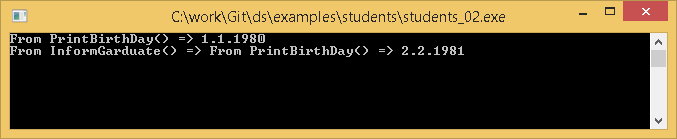
\includegraphics[scale=0.6]{images/lec06-pic19.png}
\end{figure}
\end{frame}

\begin{frame}{Преимущества использования наследования}
\begin{itemize}
\item возможность повторного использования кода (это достигается и агрегированием);
\item возможность отразить взаимоотношения объектов, свойственные предметной области;
\item возможность рассматривать производный класс как подкласс базового,
упрощая реализацию кода для производного класса;
\item возможность обработки производных классов методами, разработанными
при проектировании базового класса;
\item возможность обновления или изменения содержания этих методов применительно к объектам производного класса, если такая необходимость имеется.
\end{itemize}
\end{frame}

\begin{frame}{Обращение к одноименным методам}
\begin{figure}[h]
\centering
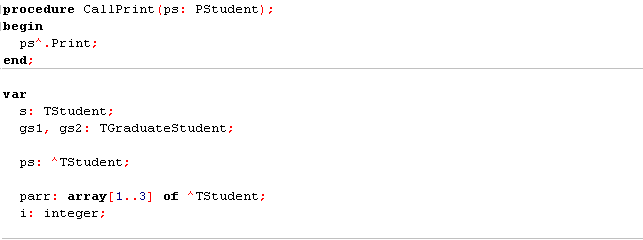
\includegraphics[scale=0.6]{images/lec06-pic20.png}
\end{figure}
\end{frame}

\begin{frame}{Обращение к одноименным методам}
\begin{figure}[h]
\centering
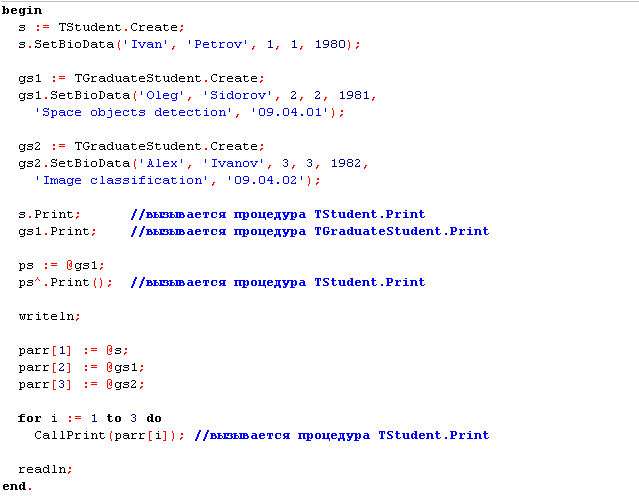
\includegraphics[scale=0.6]{images/lec06-pic21.png}
\end{figure}
\end{frame}

\begin{frame}{Обращение к одноименным методам}
\begin{figure}[h]
\centering
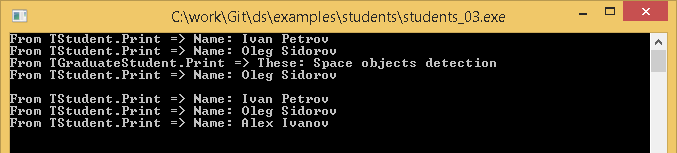
\includegraphics[scale=0.6]{images/lec06-pic22.png}
\end{figure}
\end{frame}

\subsection{Переопределение методов в производном классе}
\begin{frame}{Переопределение методов в производном классе}
Программист может переопределить унаследованную функцию-член базового класса, если содержание метода его не устраивает.
\begin{figure}[h]
\centering
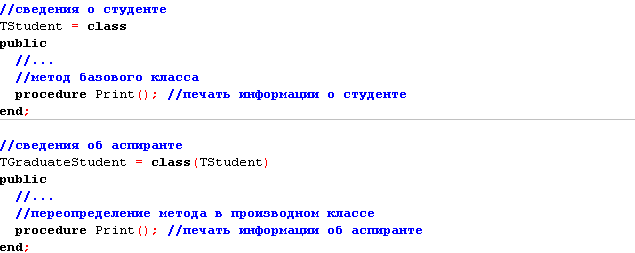
\includegraphics[scale=0.5]{images/lec06-pic23.png}
\end{figure}
При этом сохраняет возможность обратиться к методу базового класса:
\begin{figure}[h]
\centering
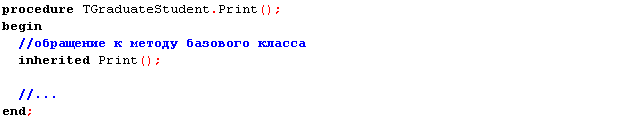
\includegraphics[scale=0.5]{images/lec06-pic24.png}
\end{figure}
\end{frame}

\begin{frame}{Инициализация объектов производного класса}
Если базовый класс имеет конструктор, он должен быть вызван. Конструкторы по умолчанию могут быть вызваны неявно. Если базовый класс не имеет
конструктора по умолчанию, следует обеспечить его явный вызов.
\begin{figure}[h]
\centering
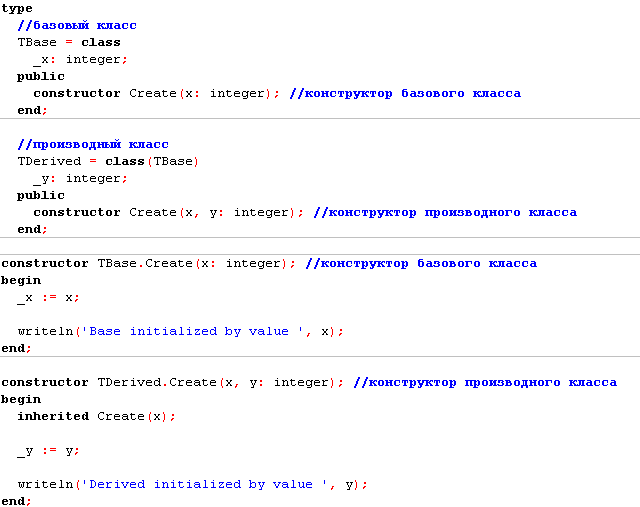
\includegraphics[scale=0.4]{images/lec06-pic25.png}
\end{figure}
\end{frame}

\begin{frame}{Инициализация объектов производного класса}
\begin{figure}[h]
\centering
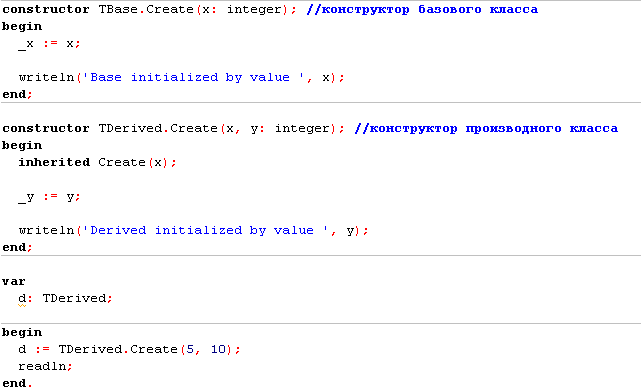
\includegraphics[scale=0.4]{images/lec06-pic26.png}
\end{figure}
В результате будет напечатано:
\begin{figure}[h]
\centering
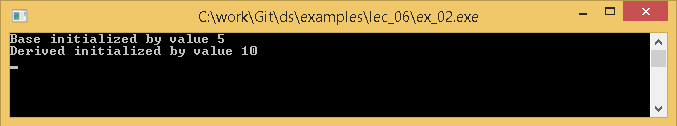
\includegraphics[scale=0.4]{images/lec06-pic27.png}
\end{figure}
\end{frame}

\begin{frame}{Порядок вызовов конструкторов и деструкторов}
\begin{figure}[h]
\centering
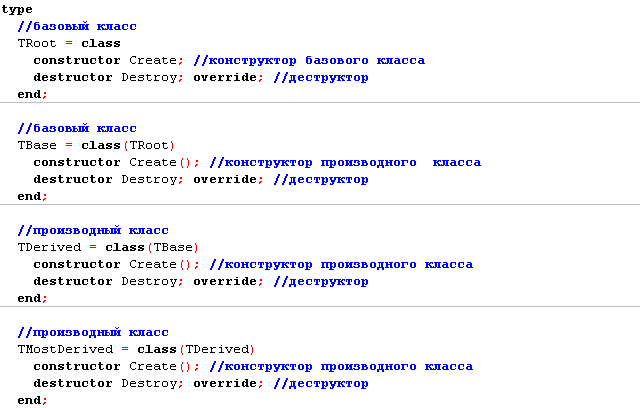
\includegraphics[scale=0.5]{images/lec06-pic28.png}
\end{figure}
\end{frame}

\begin{frame}{Порядок вызовов конструкторов и деструкторов}
\begin{figure}[h]
\centering
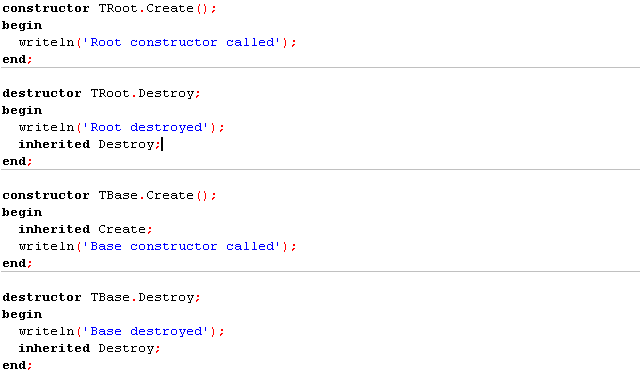
\includegraphics[scale=0.5]{images/lec06-pic29.png}
\end{figure}
\end{frame}

\begin{frame}{Порядок вызовов конструкторов и деструкторов}
\begin{figure}[h]
\centering
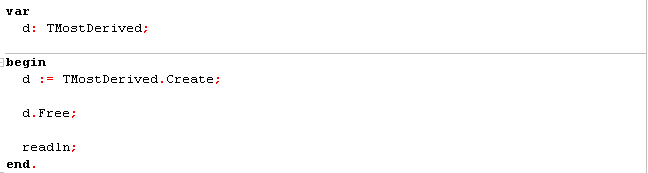
\includegraphics[scale=0.5]{images/lec06-pic30.png}
\end{figure}
\begin{figure}[h]
\centering
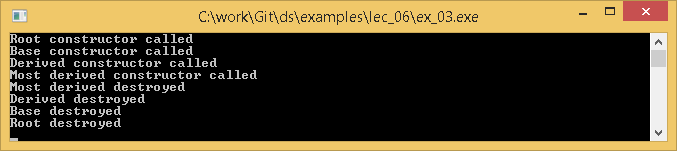
\includegraphics[scale=0.5]{images/lec06-pic31.png}
\end{figure}
\end{frame}

\subsection{Управление доступом к членам классам в связи с наследованием}
\begin{frame}{Управление доступом к членам классам в связи с наследованием}
\begin{itemize}
\item члены класса, объявленные со спецификатором public, доступны как в функциях-членах класса, так и за их пределами;
\item члены класса, объявленные со спецификатором private, доступны только в
функциях-членах класса;
\item если необходимо предоставить доступ к членам класса для функций-членов производного класса, но при этом закрыть доступ извне, используется спецификатор доступа protected.
\end{itemize}
\begin{figure}[h]
\centering
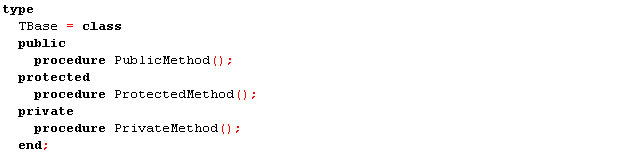
\includegraphics[scale=0.5]{images/lec06-pic32.png}
\end{figure}
\end{frame}

\begin{frame}{Управление доступом к членам классам в связи с наследованием}
\begin{figure}[h]
\centering
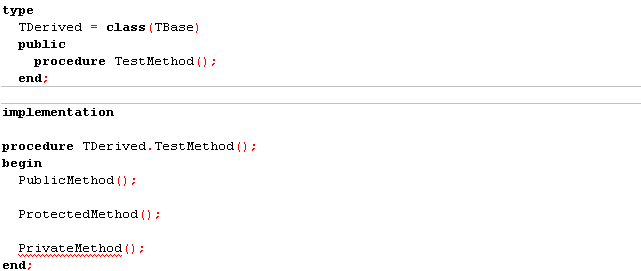
\includegraphics[scale=0.5]{images/lec06-pic33.png}
\end{figure}
\begin{figure}[h]
\centering
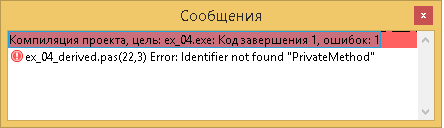
\includegraphics[scale=0.5]{images/lec06-pic34.png}
\end{figure}
\end{frame}

\subsection{Однокоренная иерархия классов}
\begin{frame}{Однокоренная иерархия классов}
\begin{block}{Однокоренная иерархия }
предполагает, что все классы неявно унаследованы (прямо или опосредованно) от
суперкласса TObject. 
\end{block}
Класс TObject определяет набор операций, общих для всех объектов. 
\begin{figure}[h]
\centering
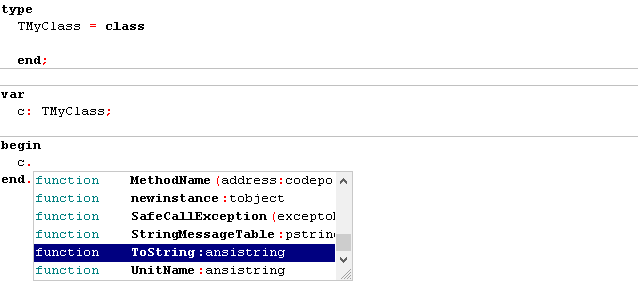
\includegraphics[scale=0.5]{images/lec06-pic35.png}
\end{figure}
Методы класса TObject могут замещаться в производных классах.
\end{frame}


\end{document}
